\documentclass[tikz,border=15pt]{standalone}
\usepackage{tikz}
\usepackage{xcolor}
\usepackage{amssymb}
\usetikzlibrary{shapes, shapes.geometric, arrows.meta, positioning,
                 fit, backgrounds, calc, shadows}

% ========== Color palette ==========
\definecolor{drawBlueFill}{HTML}{DAE8FC}
\definecolor{drawBlueLine}{HTML}{6C8EBF}
\definecolor{drawGreenFill}{HTML}{D5E8D4}
\definecolor{drawGreenLine}{HTML}{82B366}
\definecolor{drawOrangeFill}{HTML}{FFE6CC}
\definecolor{drawOrangeLine}{HTML}{D79B00}
\definecolor{drawPurpleFill}{HTML}{E1D5E7}
\definecolor{drawPurpleLine}{HTML}{9673A6}
\definecolor{drawRedFill}{HTML}{F8CECC}
\definecolor{drawRedLine}{HTML}{B85450}
\definecolor{drawGreyFill}{HTML}{F5F5F5}
\definecolor{drawGreyLine}{HTML}{666666}
\definecolor{l2Fill}{HTML}{FFF2CC}
\definecolor{l2Line}{HTML}{D6B656}
\definecolor{dramFill}{HTML}{FAD7AC}
\definecolor{dramLine}{HTML}{B46504}

\pgfdeclarelayer{background}
\pgfsetlayers{background,main}

\begin{document}
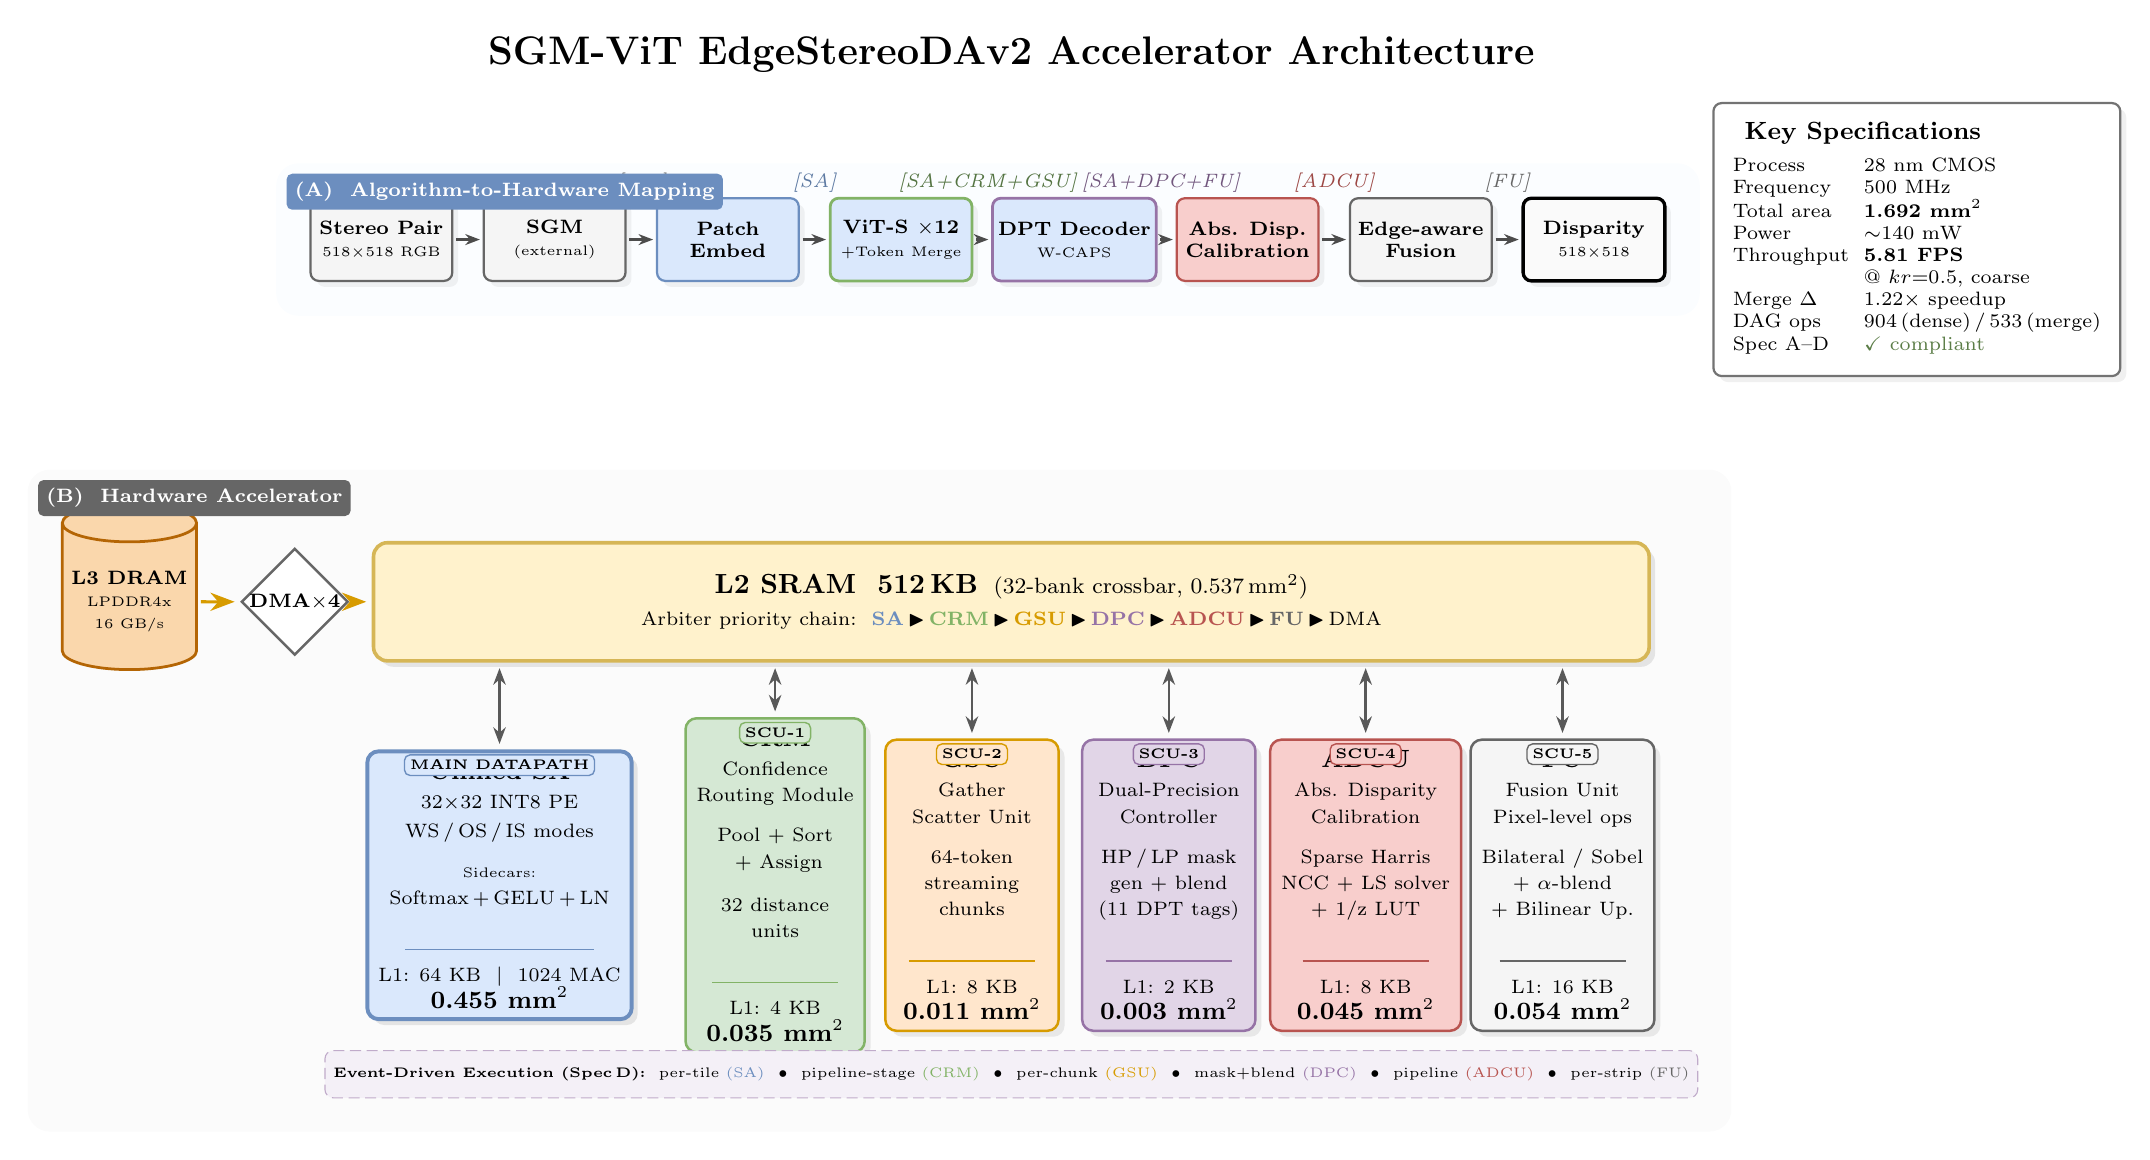
\begin{tikzpicture}[
    every node/.style={font=\footnotesize},
    sa_box/.style={rectangle, rounded corners=4pt, align=center,
        minimum width=3.2cm, minimum height=3.3cm,
        fill=drawBlueFill, draw=drawBlueLine, line width=1.4pt,
        drop shadow={opacity=0.18}, inner sep=4pt},
    scu_box/.style={rectangle, rounded corners=4pt, align=center,
        minimum width=2.2cm, minimum height=3.3cm,
        line width=0.9pt,
        drop shadow={opacity=0.15}, inner sep=4pt},
    scu_green/.style={scu_box, fill=drawGreenFill, draw=drawGreenLine},
    scu_orange/.style={scu_box, fill=drawOrangeFill, draw=drawOrangeLine},
    scu_purple/.style={scu_box, fill=drawPurpleFill, draw=drawPurpleLine},
    scu_red/.style={scu_box, fill=drawRedFill, draw=drawRedLine},
    scu_grey/.style={scu_box, fill=drawGreyFill, draw=drawGreyLine},
    l2_bar/.style={rectangle, rounded corners=5pt, align=center,
        minimum width=16.2cm, minimum height=1.5cm,
        fill=l2Fill, draw=l2Line, line width=1.3pt,
        drop shadow={opacity=0.18}, inner sep=4pt},
    dram_cyl/.style={cylinder, shape border rotate=90, aspect=0.28,
        minimum width=1.7cm, minimum height=2.1cm,
        draw=dramLine, fill=dramFill, line width=1pt, align=center,
        font=\scriptsize},
    dma_diamond/.style={diamond, draw=drawGreyLine, fill=white,
        minimum size=1.1cm, inner sep=0pt, font=\scriptsize\bfseries,
        line width=0.9pt},
    algo_node/.style={rectangle, rounded corners=3pt, align=center,
        minimum width=1.8cm, minimum height=1.05cm,
        inner sep=2pt, font=\scriptsize, line width=0.8pt,
        drop shadow={opacity=0.1}},
    spec_panel/.style={rectangle, rounded corners=3pt, align=left,
        draw=black!55, fill=white, line width=0.8pt, inner sep=7pt,
        font=\scriptsize, drop shadow={opacity=0.12}},
    badge/.style={rectangle, rounded corners=2pt, fill=white,
        inner sep=2pt, font=\tiny\bfseries, line width=0.5pt},
    data_arrow/.style={-{Stealth[scale=1.1]}, color=drawOrangeLine,
        line width=1.1pt, shorten >=2pt, shorten <=1pt},
    bidir_arrow/.style={{Stealth[scale=0.85]}-{Stealth[scale=0.85]},
        color=black!65, line width=0.9pt, shorten >=2pt, shorten <=2pt},
    algo_arrow/.style={-{Stealth[scale=0.8]}, thick, color=black!70,
        shorten >=1pt, shorten <=1pt},
    mapping_line/.style={dashed, color=black!35, line width=0.5pt,
        shorten >=1pt, shorten <=1pt},
    zone/.style={dashed, thick, inner sep=12pt, rounded corners=8pt,
        color=black!40, line width=0.9pt},
    event_strip/.style={rectangle, rounded corners=3pt,
        fill=drawPurpleFill!35, draw=drawPurpleLine!60,
        dash pattern=on 4pt off 2pt,
        minimum width=16.2cm, minimum height=0.6cm,
        align=center, font=\tiny, inner sep=3pt},
]

  % ==================== Zone A: Algorithm-to-Hardware Pipeline ====================
  \node[algo_node, fill=drawGreyFill,   draw=drawGreyLine]   (alg1) at ( 0.5, 12.5) {\textbf{Stereo Pair}\\\tiny 518$\times$518 RGB};
  \node[algo_node, fill=drawGreyFill,   draw=drawGreyLine]   (alg2) at ( 2.7, 12.5) {\textbf{SGM}\\\tiny (external)};
  \node[algo_node, fill=drawBlueFill,   draw=drawBlueLine]   (alg3) at ( 4.9, 12.5) {\textbf{Patch}\\\textbf{Embed}};
  \node[algo_node, fill=drawBlueFill,   draw=drawGreenLine,  line width=1pt] (alg4) at ( 7.1, 12.5) {\textbf{ViT-S $\times$12}\\\tiny +Token Merge};
  \node[algo_node, fill=drawBlueFill,   draw=drawPurpleLine, line width=1pt] (alg5) at ( 9.3, 12.5) {\textbf{DPT Decoder}\\\tiny W-CAPS};
  \node[algo_node, fill=drawRedFill,    draw=drawRedLine]    (alg6) at (11.5, 12.5) {\textbf{Abs. Disp.}\\\textbf{Calibration}};
  \node[algo_node, fill=drawGreyFill,   draw=drawGreyLine]   (alg7) at (13.7, 12.5) {\textbf{Edge-aware}\\\textbf{Fusion}};
  \node[algo_node, fill=drawGreyFill!50,draw=black, line width=1.2pt] (alg8) at (15.9, 12.5) {\textbf{Disparity}\\\tiny 518$\times$518};

  \foreach \a/\b in {alg1/alg2, alg2/alg3, alg3/alg4, alg4/alg5, alg5/alg6, alg6/alg7, alg7/alg8}
    \draw[algo_arrow] (\a.east) -- (\b.west);

  % Mapping labels above arrows (algorithm -> hardware modules)
  \node[font=\scriptsize\itshape, color=black!55]   at ( 3.80, 13.22) {[ext.]};
  \node[font=\scriptsize\itshape, color=drawBlueLine!85!black]   at ( 6.00, 13.22) {[SA]};
  \node[font=\scriptsize\itshape, color=drawGreenLine!65!black]  at ( 8.20, 13.22) {[SA+CRM+GSU]};
  \node[font=\scriptsize\itshape, color=drawPurpleLine!75!black] at (10.40, 13.22) {[SA+DPC+FU]};
  \node[font=\scriptsize\itshape, color=drawRedLine!85!black]    at (12.60, 13.22) {[ADCU]};
  \node[font=\scriptsize\itshape, color=drawGreyLine]            at (14.80, 13.22) {[FU]};

  % ==================== Zone B: Hardware Accelerator ====================

  % ----- Memory path: DRAM -> DMA -> L2 -----
  \node[dram_cyl] (dram) at (-2.7, 7.9) {\textbf{L3 DRAM}\\\tiny LPDDR4x\\\tiny 16 GB/s};
  \node[dma_diamond] (dma) at (-0.6, 7.9) {DMA\\$\times$4};

  % ----- L2 SRAM (hero bar) -----
  \node[l2_bar] (l2) at (8.5, 7.9) {%
    \textbf{\normalsize L2 SRAM \ 512\,KB}\ \ \textnormal{(32-bank crossbar, 0.537\,mm$^2$)}\\[2pt]
    \scriptsize Arbiter priority chain:\ \ %
    \textcolor{drawBlueLine}{\textbf{SA}}\,$\blacktriangleright$\,%
    \textcolor{drawGreenLine}{\textbf{CRM}}\,$\blacktriangleright$\,%
    \textcolor{drawOrangeLine}{\textbf{GSU}}\,$\blacktriangleright$\,%
    \textcolor{drawPurpleLine}{\textbf{DPC}}\,$\blacktriangleright$\,%
    \textcolor{drawRedLine}{\textbf{ADCU}}\,$\blacktriangleright$\,%
    \textcolor{drawGreyLine}{\textbf{FU}}\,$\blacktriangleright$\,\textnormal{DMA}%
  };

  \draw[data_arrow] (dram.east) -- (dma.west);
  \draw[data_arrow] (dma.east)  -- (l2.west);

  % ----- 6 compute modules row (y = 4.3) -----

  % SA (big, main datapath)
  \node[sa_box] (sa) at (2.0, 4.3) {%
    {\small\textbf{Unified SA}}\\[1pt]
    \scriptsize 32$\times$32 INT8 PE\\[1pt]
    \scriptsize WS\,/\,OS\,/\,IS modes\\[5pt]
    {\tiny Sidecars:}\\
    \scriptsize Softmax\,+\,GELU\,+\,LN\\[7pt]
    {\color{drawBlueLine}\rule{2.4cm}{0.4pt}}\\[2pt]
    \scriptsize L1: 64 KB\ \ $|$\ \ 1024 MAC\\
    \scriptsize \textbf{\small 0.455 mm$^2$}%
  };
  \node[badge, draw=drawBlueLine, fill=drawBlueFill] at ($(sa.north)+(0,-0.20)$) {MAIN DATAPATH};

  % CRM
  \node[scu_green] (crm) at (5.5, 4.3) {%
    {\small\textbf{CRM}}\\[1pt]
    \scriptsize Confidence\\
    \scriptsize Routing Module\\[5pt]
    \scriptsize Pool + Sort\\
    \scriptsize \ + Assign\\[6pt]
    \scriptsize 32 distance\\
    \scriptsize units\\[7pt]
    {\color{drawGreenLine}\rule{1.6cm}{0.4pt}}\\[2pt]
    \scriptsize L1: 4 KB\\
    \scriptsize \textbf{\small 0.035 mm$^2$}%
  };
  \node[badge, draw=drawGreenLine, fill=drawGreenFill] at ($(crm.north)+(0,-0.20)$) {SCU-1};

  % GSU
  \node[scu_orange] (gsu) at (8.0, 4.3) {%
    {\small\textbf{GSU}}\\[1pt]
    \scriptsize Gather\\
    \scriptsize Scatter Unit\\[5pt]
    \scriptsize 64-token\\
    \scriptsize streaming\\
    \scriptsize chunks\\[7pt]
    {\color{drawOrangeLine}\rule{1.6cm}{0.4pt}}\\[2pt]
    \scriptsize L1: 8 KB\\
    \scriptsize \textbf{\small 0.011 mm$^2$}%
  };
  \node[badge, draw=drawOrangeLine, fill=drawOrangeFill] at ($(gsu.north)+(0,-0.20)$) {SCU-2};

  % DPC
  \node[scu_purple] (dpc) at (10.5, 4.3) {%
    {\small\textbf{DPC}}\\[1pt]
    \scriptsize Dual-Precision\\
    \scriptsize Controller\\[5pt]
    \scriptsize HP\,/\,LP mask\\
    \scriptsize gen + blend\\
    \scriptsize (11 DPT tags)\\[7pt]
    {\color{drawPurpleLine}\rule{1.6cm}{0.4pt}}\\[2pt]
    \scriptsize L1: 2 KB\\
    \scriptsize \textbf{\small 0.003 mm$^2$}%
  };
  \node[badge, draw=drawPurpleLine, fill=drawPurpleFill] at ($(dpc.north)+(0,-0.20)$) {SCU-3};

  % ADCU
  \node[scu_red] (adcu) at (13.0, 4.3) {%
    {\small\textbf{ADCU}}\\[1pt]
    \scriptsize Abs. Disparity\\
    \scriptsize Calibration\\[5pt]
    \scriptsize Sparse Harris\\
    \scriptsize NCC + LS solver\\
    \scriptsize + 1/z LUT\\[7pt]
    {\color{drawRedLine}\rule{1.6cm}{0.4pt}}\\[2pt]
    \scriptsize L1: 8 KB\\
    \scriptsize \textbf{\small 0.045 mm$^2$}%
  };
  \node[badge, draw=drawRedLine, fill=drawRedFill] at ($(adcu.north)+(0,-0.20)$) {SCU-4};

  % FU
  \node[scu_grey] (fu) at (15.5, 4.3) {%
    {\small\textbf{FU}}\\[1pt]
    \scriptsize Fusion Unit\\
    \scriptsize Pixel-level ops\\[5pt]
    \scriptsize Bilateral / Sobel\\
    \scriptsize + $\alpha$-blend\\
    \scriptsize + Bilinear Up.\\[7pt]
    {\color{drawGreyLine}\rule{1.6cm}{0.4pt}}\\[2pt]
    \scriptsize L1: 16 KB\\
    \scriptsize \textbf{\small 0.054 mm$^2$}%
  };
  \node[badge, draw=drawGreyLine, fill=drawGreyFill] at ($(fu.north)+(0,-0.20)$) {SCU-5};

  % ----- Bidirectional arrows L2 <-> each module -----
  \foreach \m in {sa, crm, gsu, dpc, adcu, fu}
    \draw[bidir_arrow] (l2.south -| \m) -- (\m.north);

  % ----- Event strip at bottom -----
  \node[event_strip] (estrip) at (8.5, 1.9) {%
    \textbf{Event-Driven Execution (Spec\,D):}\ \ %
    per-tile \textcolor{drawBlueLine}{(SA)}\ \ $\bullet$\ \ %
    pipeline-stage \textcolor{drawGreenLine}{(CRM)}\ \ $\bullet$\ \ %
    per-chunk \textcolor{drawOrangeLine}{(GSU)}\ \ $\bullet$\ \ %
    mask+blend \textcolor{drawPurpleLine}{(DPC)}\ \ $\bullet$\ \ %
    pipeline \textcolor{drawRedLine}{(ADCU)}\ \ $\bullet$\ \ %
    per-strip \textcolor{drawGreyLine}{(FU)}%
  };

  % ==================== Zone C: Key Specs panel ====================
  \node[spec_panel] (spec) at (20.0, 12.5) {%
    \hspace*{0.15cm}\textbf{\small Key Specifications}\\[3pt]
    \begin{tabular}{@{}l@{\ \ }l@{}}
      Process       & 28 nm CMOS\\
      Frequency     & 500 MHz\\
      Total area    & \textbf{1.692 mm$^2$}\\
      Power         & $\sim$140 mW\\
      Throughput    & \textbf{5.81 FPS}\\
                    & \scriptsize @ $kr{=}0.5$, coarse\\
      Merge $\Delta$  & 1.22$\times$ speedup\\
      DAG ops       & 904\,(dense)\,/\,533\,(merge)\\
      Spec A--D     & \textcolor{drawGreenLine!70!black}{$\checkmark$ compliant}\\
    \end{tabular}%
  };

  % ==================== Zone frames (background layer) ====================
  \begin{pgfonlayer}{background}
    \node[zone, fill=drawBlueFill!10, fit=(alg1)(alg8)] (zoneA) {};
    \node[zone, fill=drawGreyFill!40, fit=(dram)(l2)(sa)(fu)(estrip)] (zoneB) {};
  \end{pgfonlayer}

  % ==================== Zone tags (outside, top-left) ====================
  \node[rectangle, fill=drawBlueLine, text=white, font=\scriptsize\bfseries,
        inner sep=3pt, rounded corners=2pt, anchor=north west]
        at ([xshift=4pt,yshift=-4pt]zoneA.north west)
        {(A) \ Algorithm-to-Hardware Mapping};
  \node[rectangle, fill=drawGreyLine, text=white, font=\scriptsize\bfseries,
        inner sep=3pt, rounded corners=2pt, anchor=north west]
        at ([xshift=4pt,yshift=-4pt]zoneB.north west)
        {(B) \ Hardware Accelerator};

  % ==================== Figure title ====================
  \node[font=\bfseries\Large, anchor=south] at (8.5, 14.5)
    {SGM-ViT EdgeStereoDAv2 Accelerator Architecture};

\end{tikzpicture}
\end{document}
